\documentclass{standalone}
\usepackage{tikz}
\usetikzlibrary{patterns, positioning}


\begin{document}
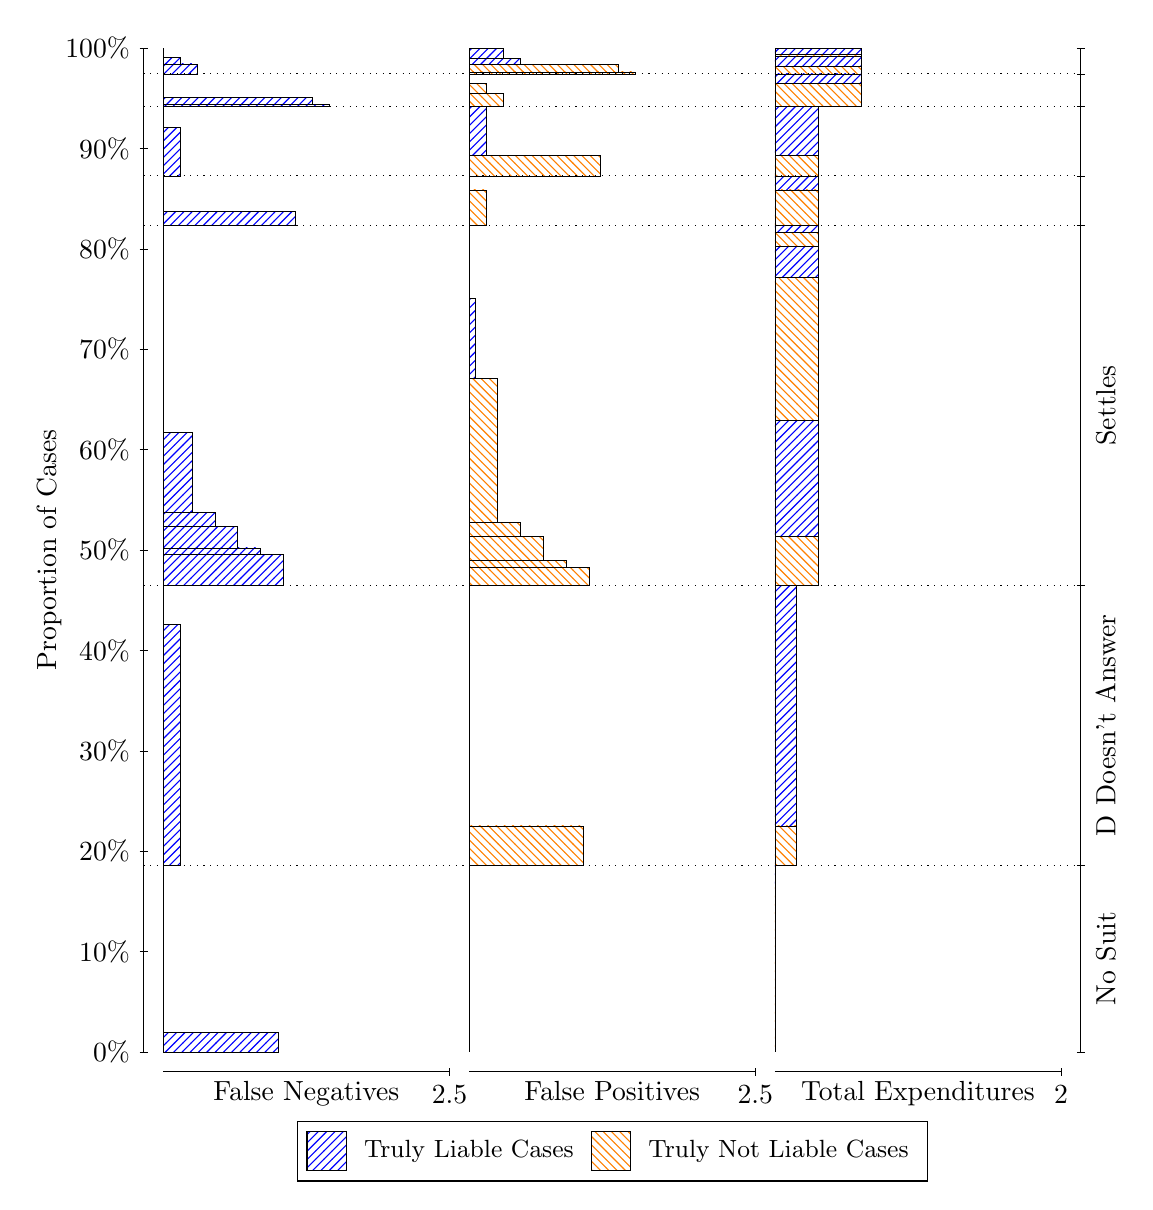
\begin{tikzpicture}
\draw[black, very thin] (1.5,1.75) -- (1.5,14.5);
\node[rotate=90, text=black, anchor=center] at (0.3, 8.125) {Proportion of Cases};
\draw[black, very thin] (1.45,1.75) -- (1.55,1.75);
\node[text=black, anchor=east] at (1.45, 1.75) {0\%};
\draw[black, very thin] (1.45,3.025) -- (1.55,3.025);
\node[text=black, anchor=east] at (1.45, 3.025) {10\%};
\draw[black, very thin] (1.45,4.3) -- (1.55,4.3);
\node[text=black, anchor=east] at (1.45, 4.3) {20\%};
\draw[black, very thin] (1.45,5.575) -- (1.55,5.575);
\node[text=black, anchor=east] at (1.45, 5.575) {30\%};
\draw[black, very thin] (1.45,6.85) -- (1.55,6.85);
\node[text=black, anchor=east] at (1.45, 6.85) {40\%};
\draw[black, very thin] (1.45,8.125) -- (1.55,8.125);
\node[text=black, anchor=east] at (1.45, 8.125) {50\%};
\draw[black, very thin] (1.45,9.4) -- (1.55,9.4);
\node[text=black, anchor=east] at (1.45, 9.4) {60\%};
\draw[black, very thin] (1.45,10.675) -- (1.55,10.675);
\node[text=black, anchor=east] at (1.45, 10.675) {70\%};
\draw[black, very thin] (1.45,11.95) -- (1.55,11.95);
\node[text=black, anchor=east] at (1.45, 11.95) {80\%};
\draw[black, very thin] (1.45,13.225) -- (1.55,13.225);
\node[text=black, anchor=east] at (1.45, 13.225) {90\%};
\draw[black, very thin] (1.45,14.5) -- (1.55,14.5);
\node[text=black, anchor=east] at (1.45, 14.5) {100\%};

\draw[black, very thin] (13.4,1.75) -- (13.4,14.5);
\draw[black, very thin] (13.35,1.75) -- (13.45,1.75);
\node[anchor=west] at (13.35, 1.75) {};
\draw[black, very thin] (13.35,4.1224) -- (13.45,4.1224);
\node[anchor=west] at (13.35, 4.1224) {};
\draw[black, very thin] (13.35,7.6783) -- (13.45,7.6783);
\node[anchor=west] at (13.35, 7.6783) {};
\draw[black, very thin] (13.35,12.246) -- (13.45,12.246);
\node[anchor=west] at (13.35, 12.246) {};
\draw[black, very thin] (13.35,12.877) -- (13.45,12.877);
\node[anchor=west] at (13.35, 12.877) {};
\draw[black, very thin] (13.35,13.756) -- (13.45,13.756);
\node[anchor=west] at (13.35, 13.756) {};
\draw[black, very thin] (13.35,14.171) -- (13.45,14.171);
\node[anchor=west] at (13.35, 14.171) {};
\draw[black, very thin] (13.35,14.5) -- (13.45,14.5);
\node[anchor=west] at (13.35, 14.5) {};

\draw[black, very thin, pattern color=blue, pattern=north east lines] (1.75,1.75) rectangle (3.2033,1.9996);
\draw[black, very thin, pattern color=orange, pattern=north west lines] (1.75,1.9996) rectangle (1.75,4.1224);
\draw[black, very thin, pattern color=blue, pattern=north east lines] (1.75,4.1224) rectangle (1.968,7.1798);
\draw[black, very thin, pattern color=orange, pattern=north west lines] (1.75,7.1798) rectangle (1.75,7.6783);
\draw[black, very thin, pattern color=blue, pattern=north east lines] (1.75,7.6783) rectangle (3.276,8.0652);
\draw[black, very thin, pattern color=blue, pattern=north east lines] (1.75,8.0652) rectangle (2.9853,8.1516);
\draw[black, very thin, pattern color=blue, pattern=north east lines] (1.75,8.1516) rectangle (2.6947,8.421);
\draw[black, very thin, pattern color=blue, pattern=north east lines] (1.75,8.421) rectangle (2.404,8.6036);
\draw[black, very thin, pattern color=blue, pattern=north east lines] (1.75,8.6036) rectangle (2.1133,9.6227);
\draw[black, very thin, pattern color=orange, pattern=north west lines] (1.75,9.6227) rectangle (1.75,12.246);
\draw[black, very thin, pattern color=blue, pattern=north east lines] (1.75,12.246) rectangle (3.4213,12.425);
\draw[black, very thin, pattern color=orange, pattern=north west lines] (1.75,12.425) rectangle (1.75,12.877);
\draw[black, very thin, pattern color=blue, pattern=north east lines] (1.75,12.877) rectangle (1.968,13.491);
\draw[black, very thin, pattern color=orange, pattern=north west lines] (1.75,13.491) rectangle (1.75,13.756);
\draw[black, very thin, pattern color=blue, pattern=north east lines] (1.75,13.756) rectangle (3.8573,13.786);
\draw[black, very thin, pattern color=blue, pattern=north east lines] (1.75,13.786) rectangle (3.6393,13.878);
\draw[black, very thin, pattern color=orange, pattern=north west lines] (1.75,13.878) rectangle (1.75,14.171);
\draw[black, very thin, pattern color=blue, pattern=north east lines] (1.75,14.171) rectangle (2.186,14.298);
\draw[black, very thin, pattern color=blue, pattern=north east lines] (1.75,14.298) rectangle (1.968,14.377);
\draw[black, very thin, pattern color=orange, pattern=north west lines] (1.75,14.377) rectangle (1.75,14.5);
\draw[black, very thin, pattern color=orange, pattern=north west lines] (5.6333,1.75) rectangle (5.6333,3.8728);
\draw[black, very thin, pattern color=blue, pattern=north east lines] (5.6333,3.8728) rectangle (5.6333,4.1224);
\draw[black, very thin, pattern color=orange, pattern=north west lines] (5.6333,4.1224) rectangle (7.0867,4.6209);
\draw[black, very thin, pattern color=blue, pattern=north east lines] (5.6333,4.6209) rectangle (5.6333,7.6783);
\draw[black, very thin, pattern color=orange, pattern=north west lines] (5.6333,7.6783) rectangle (7.1593,7.9081);
\draw[black, very thin, pattern color=orange, pattern=north west lines] (5.6333,7.9081) rectangle (6.8687,7.9946);
\draw[black, very thin, pattern color=orange, pattern=north west lines] (5.6333,7.9946) rectangle (6.578,8.298);
\draw[black, very thin, pattern color=orange, pattern=north west lines] (5.6333,8.298) rectangle (6.2873,8.4806);
\draw[black, very thin, pattern color=orange, pattern=north west lines] (5.6333,8.4806) rectangle (5.9967,10.302);
\draw[black, very thin, pattern color=blue, pattern=north east lines] (5.6333,10.302) rectangle (5.706,11.321);
\draw[black, very thin, pattern color=blue, pattern=north east lines] (5.6333,11.321) rectangle (5.6333,12.246);
\draw[black, very thin, pattern color=orange, pattern=north west lines] (5.6333,12.246) rectangle (5.8513,12.697);
\draw[black, very thin, pattern color=blue, pattern=north east lines] (5.6333,12.697) rectangle (5.6333,12.877);
\draw[black, very thin, pattern color=orange, pattern=north west lines] (5.6333,12.877) rectangle (7.3047,13.141);
\draw[black, very thin, pattern color=blue, pattern=north east lines] (5.6333,13.141) rectangle (5.8513,13.756);
\draw[black, very thin, pattern color=orange, pattern=north west lines] (5.6333,13.756) rectangle (6.0693,13.92);
\draw[black, very thin, pattern color=orange, pattern=north west lines] (5.6333,13.92) rectangle (5.8513,14.048);
\draw[black, very thin, pattern color=blue, pattern=north east lines] (5.6333,14.048) rectangle (5.6333,14.171);
\draw[black, very thin, pattern color=orange, pattern=north west lines] (5.6333,14.171) rectangle (7.7407,14.196);
\draw[black, very thin, pattern color=orange, pattern=north west lines] (5.6333,14.196) rectangle (7.5227,14.293);
\draw[black, very thin, pattern color=blue, pattern=north east lines] (5.6333,14.293) rectangle (6.2873,14.373);
\draw[black, very thin, pattern color=blue, pattern=north east lines] (5.6333,14.373) rectangle (6.0693,14.5);
\draw[black, very thin, pattern color=orange, pattern=north west lines] (9.5167,1.75) rectangle (9.5167,3.8728);
\draw[black, very thin, pattern color=blue, pattern=north east lines] (9.5167,3.8728) rectangle (9.5167,4.1224);
\draw[black, very thin, pattern color=orange, pattern=north west lines] (9.5167,4.1224) rectangle (9.7892,4.6209);
\draw[black, very thin, pattern color=blue, pattern=north east lines] (9.5167,4.6209) rectangle (9.7892,7.6783);
\draw[black, very thin, pattern color=orange, pattern=north west lines] (9.5167,7.6783) rectangle (10.062,8.298);
\draw[black, very thin, pattern color=blue, pattern=north east lines] (9.5167,8.298) rectangle (10.062,9.7691);
\draw[black, very thin, pattern color=orange, pattern=north west lines] (9.5167,9.7691) rectangle (10.062,11.59);
\draw[black, very thin, pattern color=blue, pattern=north east lines] (9.5167,11.59) rectangle (10.062,11.977);
\draw[black, very thin, pattern color=orange, pattern=north west lines] (9.5167,11.977) rectangle (10.062,12.16);
\draw[black, very thin, pattern color=blue, pattern=north east lines] (9.5167,12.16) rectangle (10.062,12.246);
\draw[black, very thin, pattern color=orange, pattern=north west lines] (9.5167,12.246) rectangle (10.062,12.697);
\draw[black, very thin, pattern color=blue, pattern=north east lines] (9.5167,12.697) rectangle (10.062,12.877);
\draw[black, very thin, pattern color=orange, pattern=north west lines] (9.5167,12.877) rectangle (10.062,13.141);
\draw[black, very thin, pattern color=blue, pattern=north east lines] (9.5167,13.141) rectangle (10.062,13.756);
\draw[black, very thin, pattern color=orange, pattern=north west lines] (9.5167,13.756) rectangle (10.607,14.048);
\draw[black, very thin, pattern color=blue, pattern=north east lines] (9.5167,14.048) rectangle (10.607,14.171);
\draw[black, very thin, pattern color=orange, pattern=north west lines] (9.5167,14.171) rectangle (10.607,14.267);
\draw[black, very thin, pattern color=blue, pattern=north east lines] (9.5167,14.267) rectangle (10.607,14.394);
\draw[black, very thin, pattern color=orange, pattern=north west lines] (9.5167,14.394) rectangle (10.607,14.42);
\draw[black, very thin, pattern color=blue, pattern=north east lines] (9.5167,14.42) rectangle (10.607,14.5);
\draw[black, dotted] (1.5,4.1224) -- (13.4,4.1224);
\draw[black, dotted] (1.5,7.6783) -- (13.4,7.6783);
\draw[black, dotted] (1.5,12.246) -- (13.4,12.246);
\draw[black, dotted] (1.5,12.877) -- (13.4,12.877);
\draw[black, dotted] (1.5,13.756) -- (13.4,13.756);
\draw[black, dotted] (1.5,14.171) -- (13.4,14.171);
\draw[black, very thin] (1.75,1.5) -- (5.3833,1.5);
\node[text=black, anchor=north] at (3.5667, 1.5) {False Negatives};
\draw[black, very thin] (5.3833,1.45) -- (5.3833,1.55);
\node[text=black, anchor=north] at (5.3833, 1.45) {2.5};

\draw[black, very thin] (5.6333,1.5) -- (9.2667,1.5);
\node[text=black, anchor=north] at (7.45, 1.5) {False Positives};
\draw[black, very thin] (9.2667,1.45) -- (9.2667,1.55);
\node[text=black, anchor=north] at (9.2667, 1.45) {2.5};

\draw[black, very thin] (9.5167,1.5) -- (13.15,1.5);
\node[text=black, anchor=north] at (11.333, 1.5) {Total Expenditures};
\draw[black, very thin] (13.15,1.45) -- (13.15,1.55);
\node[text=black, anchor=north] at (13.15, 1.45) {2};

\node[text=black, centered, rotate=90] at (13.72, 2.9362) {No Suit};
\node[text=black, centered, rotate=90] at (13.72, 5.9003) {D Doesn't Answer};
\node[text=black, centered, rotate=90] at (13.72, 9.9622) {Settles};





\draw (7.449999999999999,1.5) node[draw=none] (baseCoordinate) {};
\begin{scope}[align=center]
        \matrix[scale=0.5, draw=black, below=0.5cm of baseCoordinate, nodes={draw}, column sep=0.1cm]{
            \node[rectangle, draw, minimum width=0.5cm, minimum height=0.5cm, pattern color=blue, pattern=north east lines] {}; &
            \node[draw=none, font=\small, text=black] (B) {Truly Liable Cases}; &
            \node[rectangle, draw, minimum width=0.5cm, minimum height=0.5cm, pattern color=orange, pattern=north west lines] {}; &
            \node[draw=none, font=\small, text=black] (B) {Truly Not Liable Cases}; \\
            };
\end{scope}

\end{tikzpicture}
\end{document}